The goal of this work is to control the simulated car in CARLA using motor intent from the user's brain activity. The measured EEG contains several information and the motor intent of the user can be extracted from the Motor Imagery (MI) information. This chapter discusses different brain signal extraction methods, various EEG paradigms and components of a basic brain signal processing pipeline. Primarily the chapter focuses on brain signal extraction and removing of the artifacts in brain signals to obtain a clean feature rich signal. The methods discussed are widely researched and applied by several industries and research communities \cite{2020_Survey_DL_BCI}, \cite{2022_MI_DL_Old_Survey}, \cite{2021_Book_Deep_Learning_EEG}, \cite{2013_Book_BCI_Intro}.

\section{Brain Signal Acquisition/ Extraction}
Neurons are the basic computational unit of the nervous system. The electric signal recorded as brain waves is the result of electro-chemical interactions that occur at the outer membranes of neurons \cite{2013_Book_BCI_Intro}. In case of an event, the rise and fall of potential at the membrane of the neurons is called as action potential. The electrical activity at the neurons enables us to record and decode the brain activities. There are many ways to record the electrical activities, broadly classified into invasive and non-invasive recording. Some technologies can also be used to stimulate neurons of brain regions, which allows BCIs to send feedback to train algorithms based on interactions with the world. This work is only on Electroencephalography, a non-invasive approach, hence the topics of invasive approaches and other non-invasive approaches are explained briefly.

\subsection{Invasive Approaches}
Approaches requiring some surgery where an electrode is placed in direct contact with required region in the brain are invasive methods of recording brain signals. These approaches are typically performed on animals such as monkeys and rats. In case of humans these approaches are carried out on under strict clinical settings. As the recording sensor is in direct contact with the brain tissues, these provide higher quality signals with high SNR, higher spatial resolution and less spatial smearing compared to the non-invasive approaches.

\subsubsection{Electrocorticography (ECoG)}
ECoG \nomenclature{ECoG}{Electrocorticography}is an extra cortical invasive electro-physiological monitoring method \cite{2021_Book_Deep_Learning_EEG}. Typically performed in a clinical setting, a strip of electrodes are placed on the surface of interest on the brain. It is the most commonly used invasive approach as it has many advantages compared to other invasive approaches.

\subsection{Non-Invasive Approaches}
Approaches that gather brain signals over the surface of the scalp, without any surgery or electrodes being inserted into the skull are termed non-invasive approaches. The signals could be collected by measuring the electrical or magnetic activity on the surface of the scalp. Some of the common non-invasive approaches are Electroencephalography (EEG)\nomenclature{EEG}{Electroencephalography}, functional magnetic resonance imaging (fMRI), functional near-infrared spectroscopy (fNIRS), magnetoencephalography (MEG), and electrooculography (EOG)\nomenclature{EOG}{Electrooculography}.
    
%     \subsubsection{Functional Near-infrared Spectroscopy (fNIRS)}
% fNIRS uses near-infrared light to measure the degree of oxygenated and deoxygenated haemoglobin. The relative levels 

\subsubsection{Electroencephalography (EEG)}
EEG is the most commonly used non-invasive approach used to measure brain electrical activity on the surface of the scalp. The electrodes are usually placed according to the internationally recognized 10-20 system (see figure \ref{fig:10_20}). In this work the electrode names and its locations are slightly off and it is given in \ref{fig:obci_eegpose} \cite{1020_system_oci}. The spatial resolution of the signals depend on the number of electrodes used. The temporal resolution depends on how many samples the system could measure in a second. Typically the temporal resolution of the EEG signals is much better than the spatial resolution. In comparison to invasive approaches, the EEG systems have poor spatial and temporal resolution, and very poor SNR\cite{2013_Book_BCI_Intro}. Since the measurement is taken over the surface of the scalp, the obstruction of the skull and other tissues between cortex and the scalp act as a huge conductive surface leading to spatial smearing. However with other non-invasive approaches, EEG has higher temporal resolution, tolerance to noise and artifacts, low cost and no exposure to high intensity magnetic fields.

\begin{figure}[H] 
    \begin{center}
    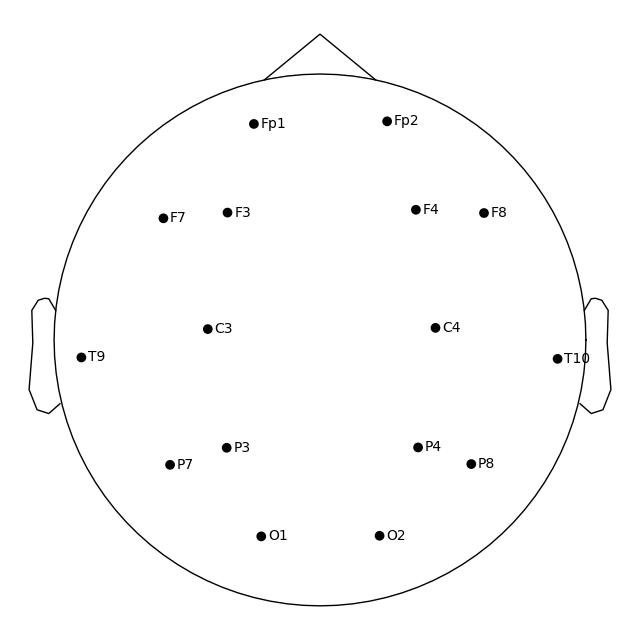
\includegraphics[height=0.6\textwidth]{images/obci_eegpose.png}
    \caption{Electrode positioning used in this work}
    \label{fig:obci_eegpose}
\end{center}
\end{figure}

\begin{figure}[H] 
    \begin{center}
    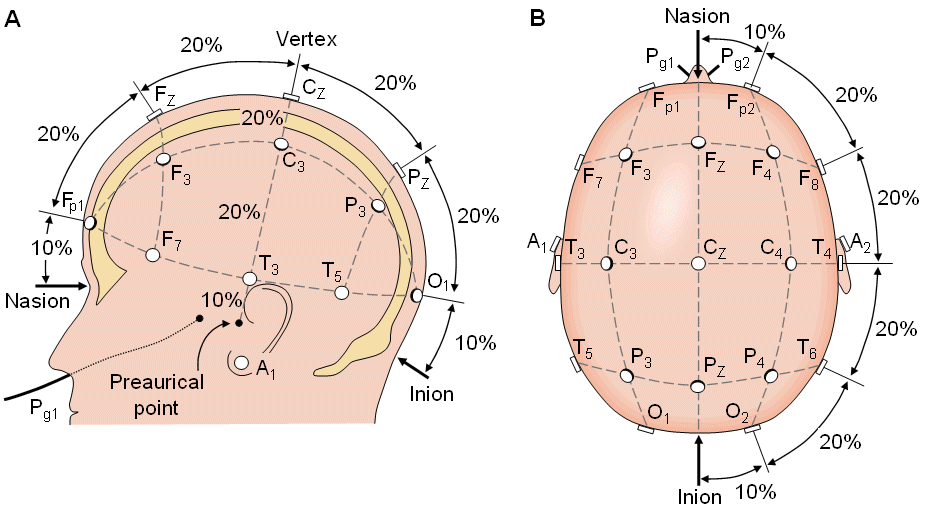
\includegraphics[height=0.6\textwidth]{images/10_20.png}
    \caption{10-20 system of internationally accepted electrode placement. Source \cite{1020_system}}
    \label{fig:10_20}
\end{center}
\end{figure}

Spatial smearing is the effect by which all the electrodes tend to measure the same signal because of the conductive effect of the tissues between the cortex and scalp. EEG signals also very susceptible to other noises such as power-lines, changing electrode impedance, eye movements, eye blinks, facial muscle movements and head movement\cite{2013_Book_BCI_Intro}. The brain signals measured from the EEG systems can be separated into frequency bands, where each frequency band represents a specific brain state and level of awareness. The recorded brain signals contain information on various physiological, psychological, mental, sensory and cognitive activities. Hence it is required to analyse and extract the relevant information from the signal.

\section{EEG Paradigms}
The measured EEG data is rich in information relating to several human conscious and subconscious activities. In case of a controlled lab experiments, the brain signals are recorded with few stimuli and feedback requiring the focus of the user. Depending on the type of experiment and the task that is required to achieve, the brain signal analysis methods vary. These experiments are designed to utilize neuro-physiological activities that are broadly classified into Spontaneous EEG and Evoked Potential.

\subsection{Spontaneous EEG}
Spontaneous EEG also referred as Oscillatory Activity includes a wide range of tasks typically without any external stimulation such as mental task, motor imagery, sleeping, or under fatigue stage. BCI systems that work with spontaneous EEGs are also called Active BCI as they require consciously controlled thought independent from external events. BCI systems that work with spontaneous EEG are hard to train given their low SNR and variation in subjects.

\subsubsection{Motor Imagery (MI)}
Imagining a motor(physical) movement without performing an actual movement is termed Motor Imagery. It is one of the widely researched EEG paradigms that is used in several applications where the user is limited in their motor movement capabilities. The Sensorimotor rhythms (SMRs)\nomenclature{SMR}{Sensorimotor Rhythm} are oscillatory events in the EEG signal originating from regions of the brain associated with control and action of a movement \cite{2019_BMI_MIEEG}. Gamma $\gamma$ activity can be used in case of invasive BCI systems, but it is not suitable for non-invasive systems as they do not reach the scalp. It also helps in mental rehearsals as the person experiences themselves performing the action. MI is due to two basic phenomena that occur in the brain onset of imagination - Event Related Desynchronization (ERD) and Event Related Synchronization (ERS). ERD/ERS refers to phenomena that the magnitude and the frequency distribution of the EEG signal power changes during a specific brain state. It is mostly observed in sensory, cognitive and motor tasks. During motor imagery contra-lateral ERD is observed in the $\mu$ rhythm and after motor imagery ERS is observed in $\beta$ band. The commonly used different frequency ranges for brain signal analysis is given in the table \ref{tb:freq_ranges}.


\begin{table}[H]
\centering
\arrayrulecolor{black}
\begin{tabular}{!{\color{black}\vrule}l!{\color{black}\vrule}l!{\color{black}\vrule}l!{\color{black}\vrule}} 
\hline
Frequency Band Name & Frequency Bandwidth (Hz) & State Associated with bandwidth                                                           \\ 
\hline
Delta               & 0.5 - 3.5                & Deep Sleep                                                                                \\ 
\hline
Theta               & 4 - 7.5                  & Drowsy                                                                                    \\ 
\hline
Alpha (or mu)       & 8 - 12                   & Relaxed                                                                                   \\ 
\hline
Beta                & 13 - 30                  & Engaged                                                                                   \\ 
\hline
Gamma               & 30 - 100                 & \begin{tabular}[c]{@{}l@{}}short- term memory and\\multisensory integration\end{tabular}  \\
\hline
\end{tabular}
\caption{\label{tb:freq_ranges} EEG Frequency bands.}
\arrayrulecolor{black}
\end{table}

Event Related Desynchronization (ERD) is due to activity of small set of neurons. A visual stimulation results in a short lasting attenuation or blocking of rhythm in the alpha band leading to power decrease of ongoing EEG signals. This decrease in the oscillatory is related to internally or externally paced events.

Event Related Synchronization (ERS) is due to activity of large set of neurons. The increase in oscillatory activity is again related to internally or externally paced events. It is characterized by short lasting amplitude enhancement.

\subsection{Evoked Potential (EP)}
The potentials observed in the brain signals as a result of physical stimulus rather than higher processes that might involve memory and attention. BCI systems that work with EPs \nomenclature{EP}{Evoked Potential}could be also called Reactive BCI as they rely on response to the stimulus provided. Few of the commonly researched EPs are described below.

\subsubsection{Event Related Potential (ERP)}
It is the most widely researched EPs and it is further classified based on the stimulus used to trigger the brain waves: visual evoked potential when stimulated visually, auditory evoked potential when stimulated with sound and somatosensory evoked potential when evoked with smell. The stimulus could be internal or external based on the BCI system. P300 is the the positive peak that appears 300ms after the onset of the stimulus. It is an important component in ERP and widely used in many BCI systems existing in the market.

\subsubsection{Error Related Potential (ErRP)}
It is a result of an erroneous event generated by the error processing mechanism in the human brain. It provides a feature rich feedback to the BCI system and helps to tune the system in the desirable way.

\section{Brain Signal Processing Pipeline}
The brain signal is fed through several signal processing algorithms to extract the best possible information. These processing algorithms are specifically chosen to extract motor imagery data. The overall processing pipeline is given in the figure \ref{fig:MT_Overall}. The first few steps in the processing pipeline are the same for both conventional and deep learning approaches. The variation is observed only at feature extraction and classification. These steps involved in the pipeline are explained in detail in the following sections and chapters. The data obtained needs to be processed effectively to get the best possible information as it influences the classification result dramatically. Most of the BCI systems in the literature \cite{2020_Survey_DL_BCI}, \cite{2022_MI_DL_Old_Survey}, \cite{2022_MI_classification}, \cite{2022_EEG_MI_Survey} use the following techniques to achieve the best results. 

\subsection{Data Extraction}
The input to the pipeline could be an online/offline data from OpenBCI headgear or publicly available open-source datasets. The open-source data sets were used in order to design the pipeline and later the pipeline is calibrated to work with data from the OpenBCI headgear.

\subsubsection{OpenBCI headgear}
Before the experiment could be started several parameters are checked. In order to ensure the contact of electrodes on the user's scalp, the impedance at the electrodes is monitored and adjusted until they fall into acceptable threshold i.e. less than $750K\Omega$. Next the frequency filters are configured to avoid DC offset and electric power line noises. However this filter is applied only to the visualizer and not to the recorded data. The electrodes are very susceptible to noises from electronic devices that appear around 25 Hz even after filtering the DC offset and power line noises. Hence while performing the experiment the user is expected to be away from any electronic device. In experiments, it is also proven that removal of the noise from the electronic devices is not necessary when working with deep learning based signal processing pipeline. The raw extracted and frequency band-pass filtered data is displayed in the figure \ref{fig:obci_rawfltrd}.

 \begin{figure}[H]
    \begin{center} 
    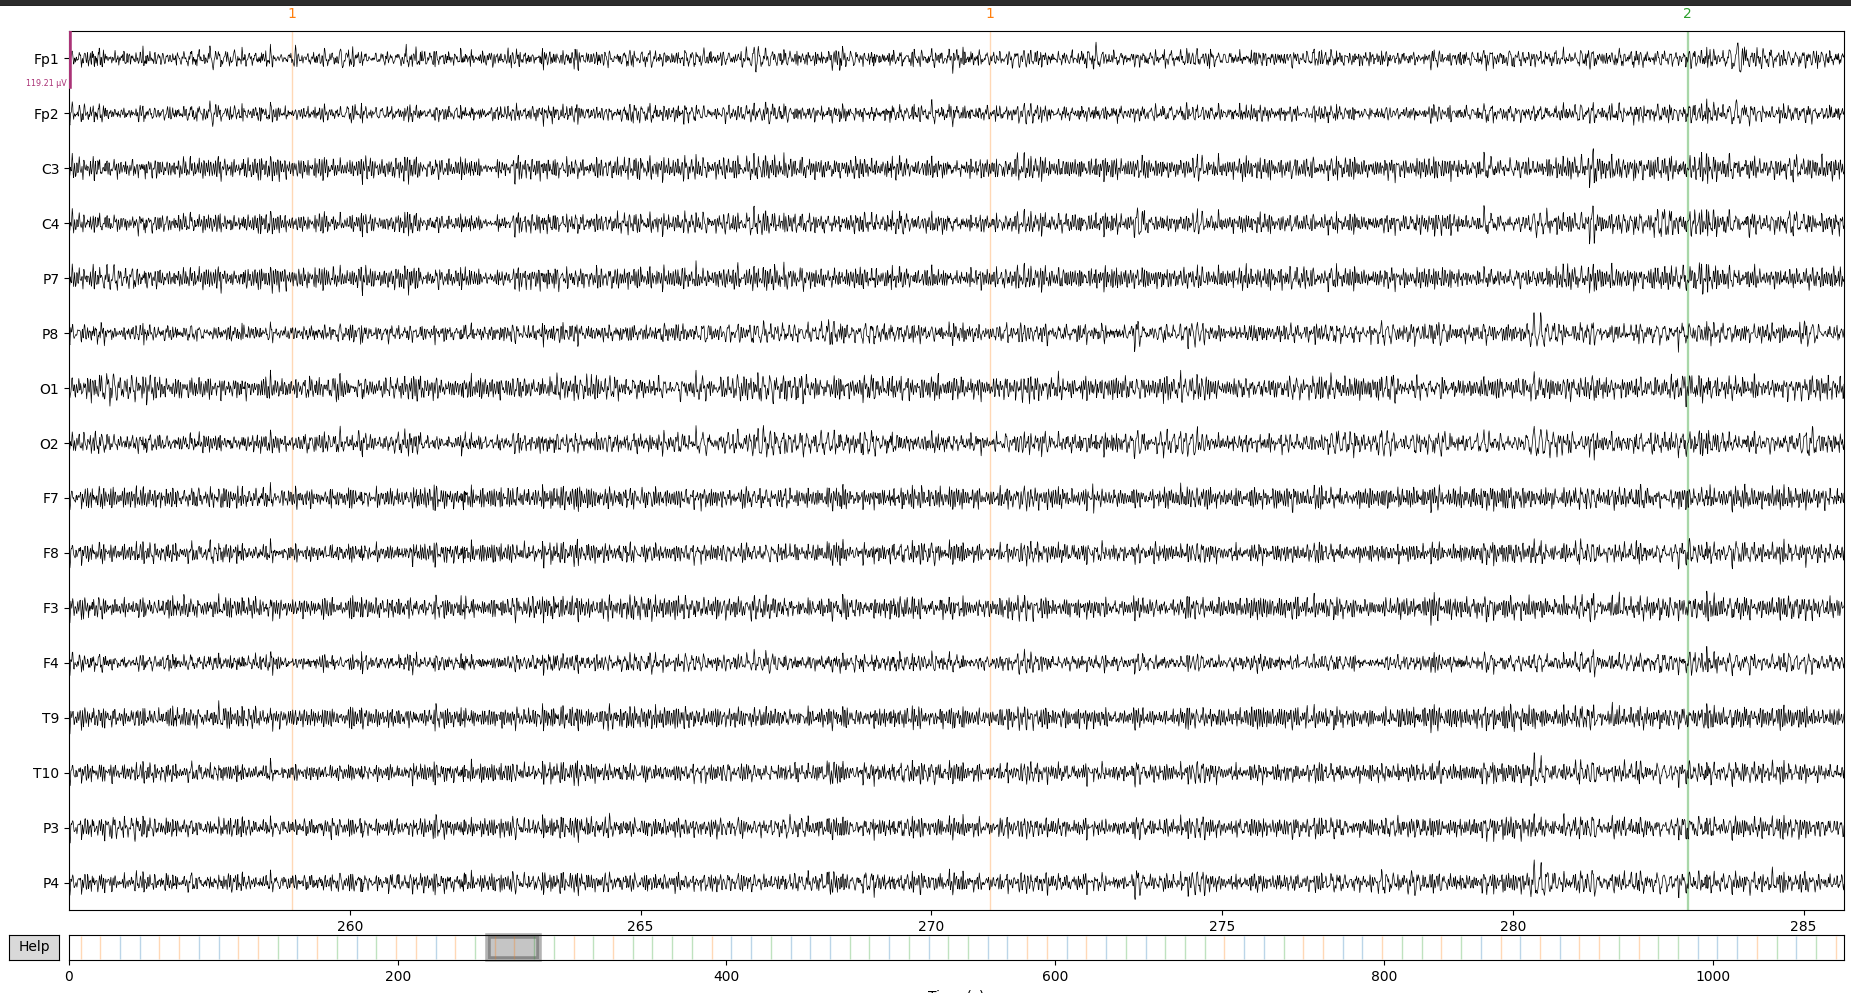
\includegraphics[height=0.6\textwidth]{images/obci_rawfltrd.png}
    \caption{Raw data(filtered) measured from OpenBCI headgear}
    \label{fig:obci_rawfltrd}
\end{center}
\end{figure}

Establishing a proper experiment is a key step in training the classifiers, By \cite{2021_MI_DCNN} each trail is recorded for 12 seconds (see figure \ref{fig:experiment}), the setup is used to gather data for a three class system that consists of a window separated by a vertical line and two squares - yellow and blue, initially in the centre. The beginning of each trial is marked by a change in color of the vertical line then the subject is requested to be in an idle state for the first 5 seconds. The motor imagery task to be performed is presented on the screen  for 3 seconds with help of a yellow square by moving it to the left, right or standstill denoting only straight motion without steering, here the subject can prepare themselves \ref{fig:experiment}. After which the subject either performs the instructed movement or imagines performing the movement for 3 seconds. The data collected so far could be used to train a model online or it can used as input to a pre-saved model and obtain the classification result. The result of the classifier is used to move the blue square accordingly. The answer presented to the subject stimulates feedback in the user which is again captured in the recording for analyzing ErRP and to improve the classifier results. The experimental setup is presented in figure \ref{fig:exp_setup}.

\begin{figure}[H] 
    \begin{center}
    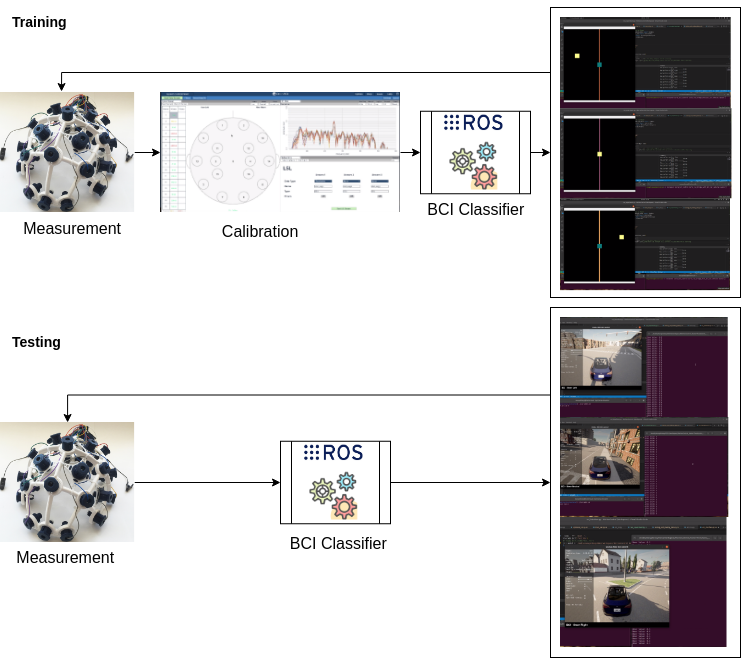
\includegraphics[height=0.6\textwidth]{images/exp_setup.png}
    \caption{Testing and Training workflow used in this work}
    \label{fig:exp_setup}
    \end{center}
\end{figure}

\begin{figure}[H] 
    \begin{center}
    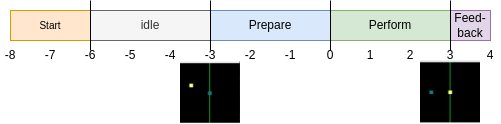
\includegraphics[width=0.8\textwidth]{images/experiment.png}
    \caption{Experimental Paradigm}
    \label{fig:experiment}
    \end{center}
\end{figure}

LSL is used to establish communication between OpenBCI GUI and CARLA BCI Control ROS node. With the support of MNE, a mock LSL stream can be used to stream recorded data which helps in debugging the algorithm even in the absence of the OpenBCI headgear.

\subsubsection{Open-source Data sets}
BCI is a widely researched field for several decades, however the huge variation in the BCI experiments to obtain relevant information from the brain signal is a bottleneck in the publicly available dataset. This work required a multi-class motor imagery dataset recorded with a 16+ channel BCI system and sampling rate of greater than 125 Hz. Some of the datasets that are used in setting up the signal processing pipeline and used for comparative analysis are discussed further. The dataset thus used were re-sampled, channel-picked in order to develop a signal processing pipeline compatible to the hardware in hand.

\subsubsection{PhysioNet}
PhysioNet dataset\cite{2004_Physionet} consists of over 1500 one- and two-minute EEG recordings from 109 participants performing motor imagery tasks using a 64-channel BCI2000 system at a sample rate of 160 Hz. Each participant performed 14 experiments each involving either imagining or actually performing opening and closing fists and feet. The PhysioNet dataset followed the international 10-20 system making it easy to construct MNE Raw frame.

\subsubsection{Berlin BCI Competition (BBCI)}
BBCI \cite{2004_BBCI} competition was held for few years where the competitors had to come up with the best performing signal processing pipeline for the given dataset. This includes a list of various EEG datasets. This work uses the motor imagery dataset from BBCI III IVa. The recordings were performed using a 118-channel EEG system at a sampling rate of 1000 Hz. It consists of 5 participants, each performing motor imagination of right fist or foot. The electrode locations in the BCI system is arbitrary and the location info was provided with the dataset. It required manual assignment of locations to enable all the functionalities in the MNE framework. From this point the word- dataset and data are used interchangeably and it is used to denote the data obtained from the OpenBCI headgear and the open-source datasets unless specified.

\subsection{Artifact removal techniques}
Any undesirable signals that originate outside the brain are termed artifacts. Techniques that are used to remove such artifacts from relevant data are effective on one such artifact. Some of the artifacts and the removal techniques described below are proven to be effective for this work. The list of algorithms is given in the diagram \ref{fig:Algorithm_overview}.

\begin{figure}[H] 
    \begin{center}
    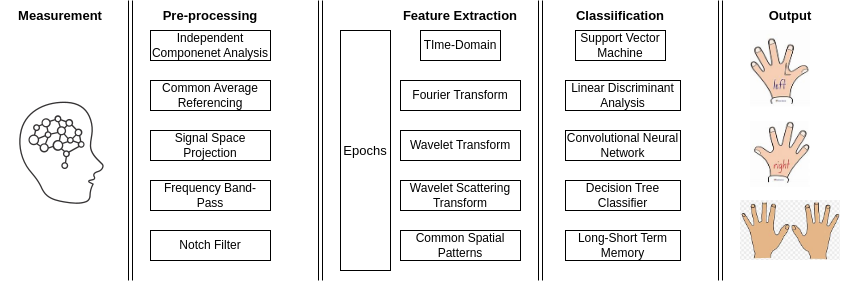
\includegraphics[width =1.0\textwidth]{images/Algorithm_overview.png}
    \caption{List of all the algorithms used.}
    \label{fig:Algorithm_overview}
    \end{center}
\end{figure}

\subsubsection{Band Pass}
The information required to perform motor imagery classification is present in the low frequency region i.e 30 Hz, hence band-passing the signal between 5 Hz and 40 Hz removes the DC offset and irrelevant information. It also avoids the need for a notch filter at 50 Hz or 60 Hz to remove the electric power line noise. The band-passed power spectral density of the recorded data is given in \ref{fig:obci_rawfltrd_psd}. The color scheme represents the location of the electrodes. In a normal indoor experimental setup the OpenBCI hardware tends to pick up several noises from the surrounding electronic devices and hence a peak is observed at 25 Hz. This does not appear in case of PhysioNet dataset \ref{fig:phy_rawfltrd_psd} as it is recorded in a laboratory environment.

\cite{2017_MI_ML_SP} proposed an approach for MI BCI system which pre-processes the data with channel selection, band-pass filtering and spatial filtering. The measured data is band-passed between 7 and 30 Hz to extract the $\mu$ and $\beta$ rhythms.

\begin{figure}[H] 
   
    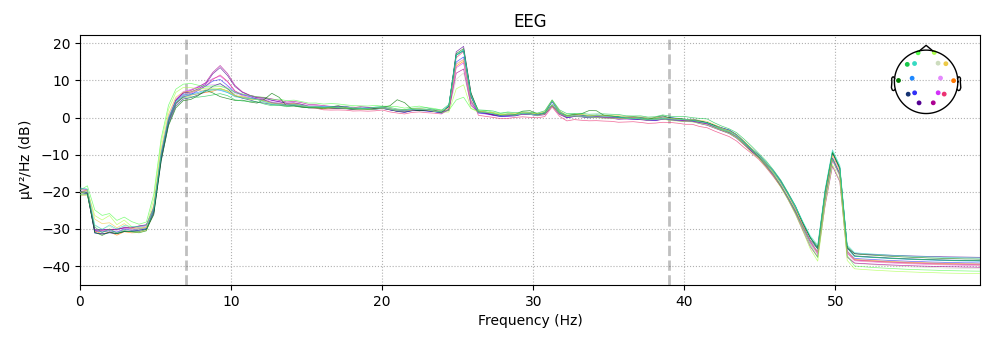
\includegraphics[width =1.0\textwidth]{images/obci_rawfltrd_psd.png}
    \caption{Power Spectral Density of brain recording obtained from OpenBCI headgear}
    \label{fig:obci_rawfltrd_psd}

\end{figure}

\begin{figure}[H] 
    \begin{center}
    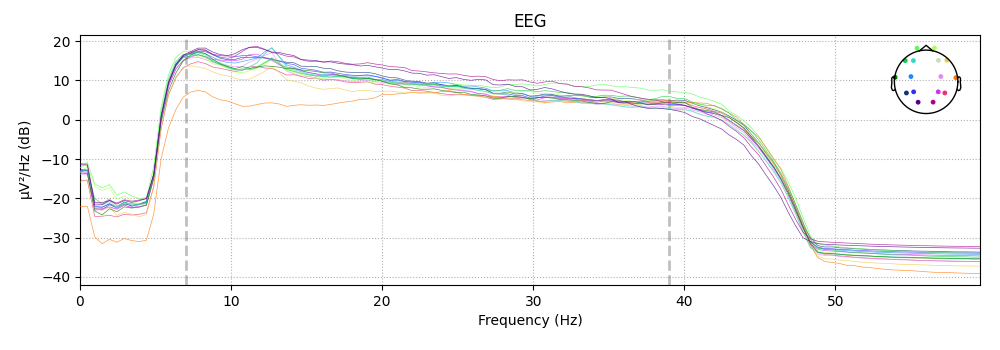
\includegraphics[width =1.0\textwidth]{images/phy_rawfltrd_psd.png}
    \caption{Power Spectral Density of brain recording obtained from PhysioNet dataset}
    \label{fig:phy_rawfltrd_psd}
\end{center}
\end{figure}

\subsubsection{Spatial Filtering}
The potential that is measured at an electrode is overlap or a linear combination of several sources in the brain. This is primarily due to volume conduction. \cite{2017_EEG_SF} proposed two spatial filtering techniques based on CSP and Fuzzy sets, and the results were shown to be better than the conventional methods. Methods like CSP require large amount of labelled data. \cite{2012_SF_MI_ICA} proposed a zero-training method to construct spatial filters for extracting changes in motor imagery information in the measured EEG signal.

Given $x_{i}$ from n independent sources, the sum of all independent sources can be written as \ref{eq:spat_smear}.
\begin{equation} \label{eq:spat_smear}
    \mathbb{C}^{j} = \sum_{n = i}^{n} w_{i}^{j} x_{i} = \mathbb{W^{j} X} 
\end{equation}

where $\mathbb{C}^{j} $ refers to measurement from arbitrary channel $j$,  $\mathbb{W^j}$ represents the weight matrix for channel $j$ and $\mathbb{X}$ represents independent sources. Inherently brain signals are low in SNR, improving the SNR would enable increased classification accuracy. Spatial filtering achieves this by performing one of the following: enhance local activity, reduce noise across channels, reduce dimensionality, identify hidden sources, find projections that maximize discrimination between different classes. The following techniques perform one of the above mentioned operations. Spatial Filters also help to invert measurement to the original source.

\paragraph{Bipolar Referencing}
Re-referencing the measurement from the electrodes is one of the common methods that help to achieve better SNR.
For a primitive system, Bipolar re-referencing will highlight the required features by finding the potential difference between two electrodes of interests. Consider measurement from channels $i$ and $j$

\begin{equation} \label{eq:bip_eeg}
    \mathbb{C}^{i}_{Bi} =  \mathbb{C}^{i} - \mathbb{C}^{j}
\end{equation}

\paragraph{Laplacian Referencing}
Laplacian re-referencing enhances local activity at the electrode of interest by subtracting the potential of the channel of interest from the potentials of the adjacent four channels $\theta$. This is achieved by removing the muscle activity from the electrode of interest.

\cite{2005_MI_TF_ICA_DipAna} uses surface Laplacian method for high-pass spatial filtering.

\begin{equation} \label{eq:lap_eeg}
    \mathbb{C}^{i}_{LP} =  \mathbb{C}^{i} - \frac{1}{4} \sum_{i \epsilon \theta} \mathbb{C}^{i}
\end{equation}

\paragraph{Common Average Referencing (CAR)}
It is the most common method of re-referencing. It is very similar to Laplacian re-referencing, but instead of the adjacent electrodes, the average of potentials of all the electrodes is subtracted. However problems can be caused in the calculation of electrode's average due to finite sample density and inadequate head coverage of EEG \cite{2022_MI_DL_Old_Survey}. The Raw data with CAR projections removed is shown in figure \ref{fig:obci_car}.

\begin{equation} \label{eq:car_eeg}
    \mathbb{C}^{i}_{CAR} =  \mathbb{C}^{i} - \frac{1}{N} \sum_{n = 1}^{N} \mathbb{C}^{i}
\end{equation}

\begin{figure}[H] 
    \begin{center}
    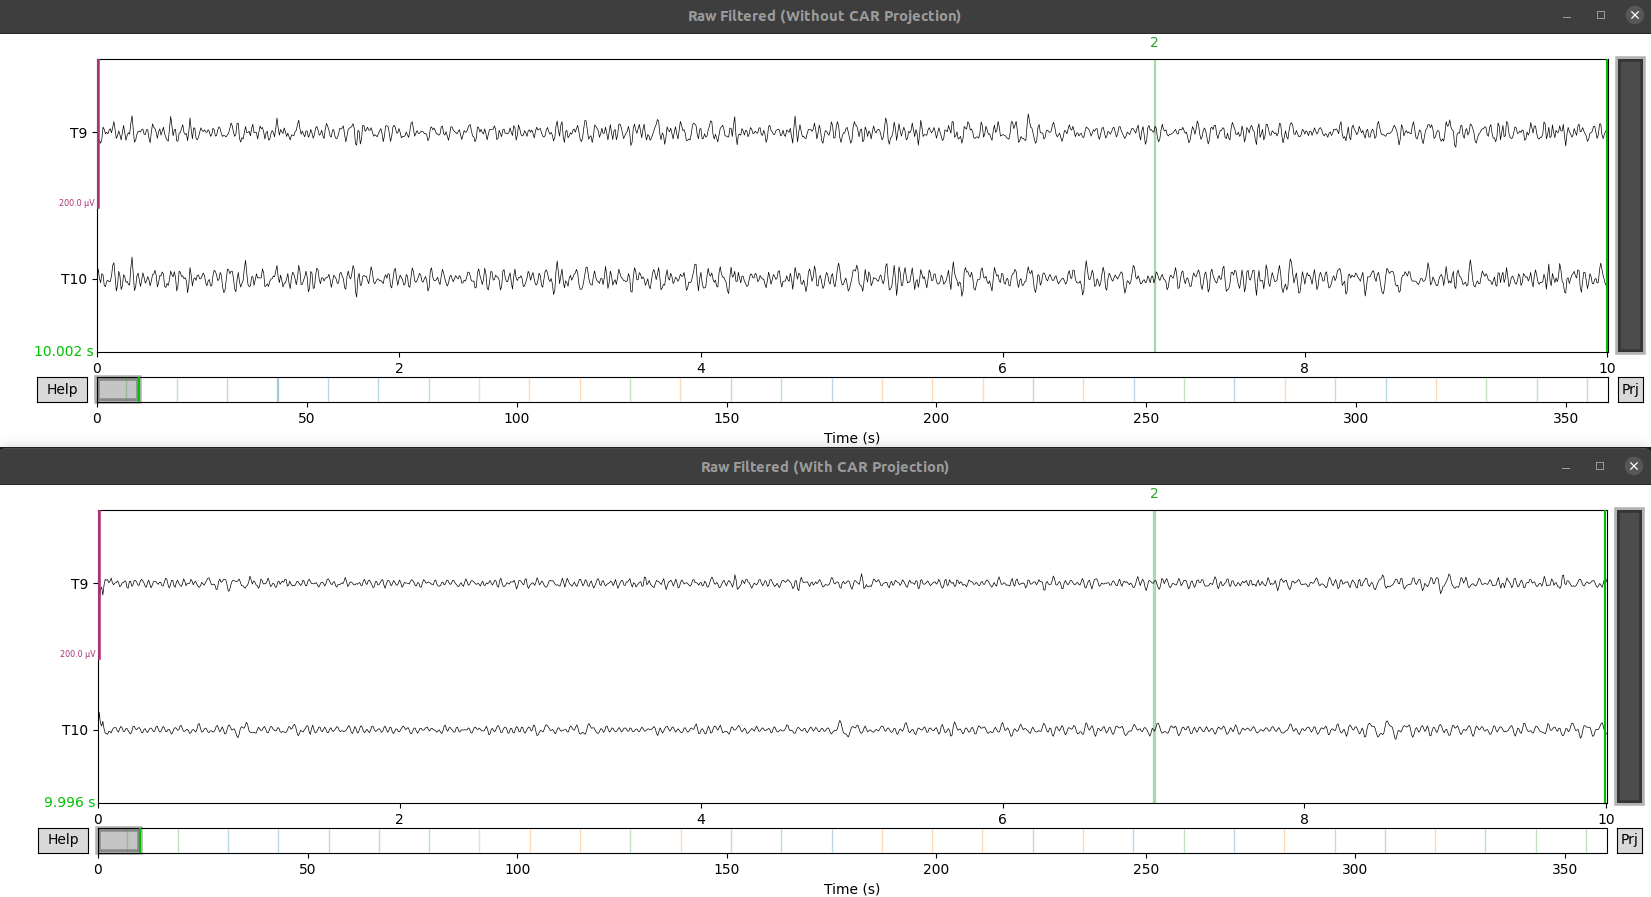
\includegraphics[height=0.6\textwidth]{images/obci_car.png}
    \caption{CAR projection applied on the EEG recording obtained from OpenBCI. The first image is before the application of the CAR projection and the second image is after application of CAR projection.}
    \label{fig:obci_car}
\end{center}
\end{figure}

\subsubsection{Independent Component Analysis (ICA)}
The potentials recorded using EEG electrodes appear the same and it is highly correlated. This measurement is highly redundant as it doesn't provide any distinctive features that could enable efficient classification. Principal Component Analysis (PCA) \nomenclature{PCA}{Principal Component Analysis} enables dimensionality reduction that helps to remove the redundant information by finding the dimensions of highest variance, also called as principal components and transforming the measured data to the directions of N desired principal components that contains the most valuable information. With reduced dimensionality the classifier can be trained effectively as the principal components serve as feature vectors as they have the necessary information. \cite{2020_MI_PCA} uses multi-scale principle component analysis for de-noising and successive decomposition index was used to extract features.

\cite{2017_MotionCOntrol_MI_ICA} proposed a BCI system to control a four wheeled electric vehicle using motor imagery. ICA was used to pre-process the raw data and then the relevant features were extracted using Common Spatial Pattern (CSP). Finally the classification was performed using a fully connected neural network. The control was limited to left or right steering command, hence the classification was binary.

\cite{2021_Feat_MI_TF_ICA_SVM} used ICA as a feature extraction method to extract the source of the measured signals and classify the motor imagery information.

Though the transformed data is decorrelated, the higher orders of the data are still dependent, i.e. the transformed data is not completely independent. For analysis of brain signals, the measured data is assumed to be a linear combination of statistically independent signals from different regions in the brain, hence complete independence of the data is essential.

Consider $\mathbb{X}$ independent sources, the measurement $\mathbb{C}$ at the channels is mixed up by mixing matrix $\mathbb{M}$ \ref{eq:mixed_ica}.

\begin{equation} \label{eq:mixed_ica}
    \mathbb{C} = \mathbb{MX} 
\end{equation}

ICA \nomenclature{ICA}{Independent Component Analysis}helps to recover the independent sources by finding the unmixing matrix $\mathbb{M^{-1}}$ \ref{eq:unmixed_ica} in case where the $n$ independent sources and $N$ channels are the same.

\begin{equation} \label{eq:unmixed_ica}
    \mathbb{X} = \mathbb{M^{-1}C}
\end{equation}

However the independent sources $\mathbb{X}$ obtained from ICA can be less than, more than or equal to the number of measured channels and not orthogonal to each other unlike PCA. It is computationally efficient and the independent components serve as feature vector for classification or removes the artifacts from the measurement. The ICA components figure \ref{fig:obci_ica_components} provides topographical information on the origin of each independent component. The number of components can be modified in the analysis, however it is lesser than the number of electrodes used in the measurement. 

\begin{figure}[H] 
    \begin{center}
    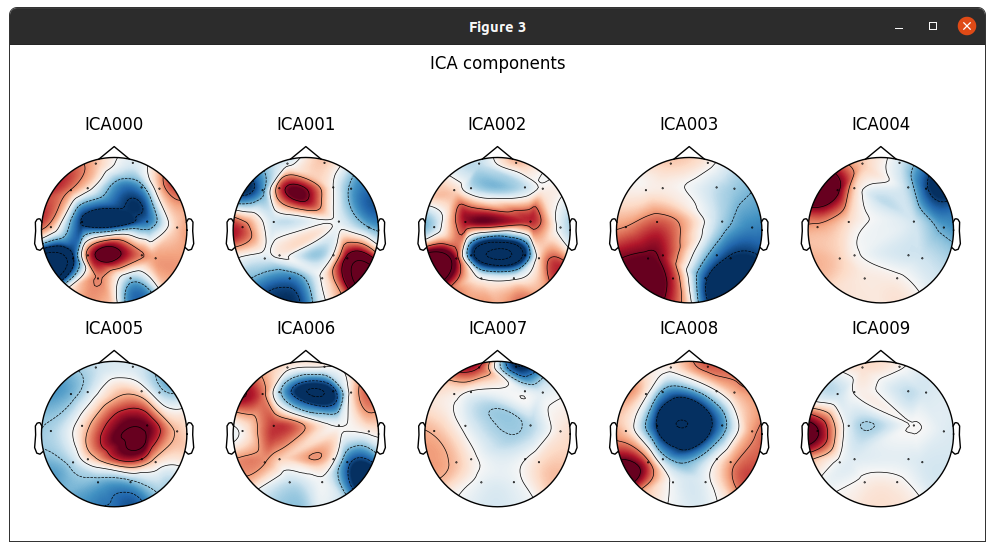
\includegraphics[width=0.8\textwidth]{images/obci_ica_components.png}
    \caption{ICA components from OpenBCI recording}
    \label{fig:obci_ica_components}
\end{center}
\end{figure}

As EEG measurements are very susceptible to eye movements, the electrodes \textit{Fp1} and \textit{Fp2} are used as references and the score plot \ref{fig:obci_ica_scores} describe how well the components relate to an artifact, which in this case is the eye movement.

\begin{figure}[h] 
    \begin{center}
    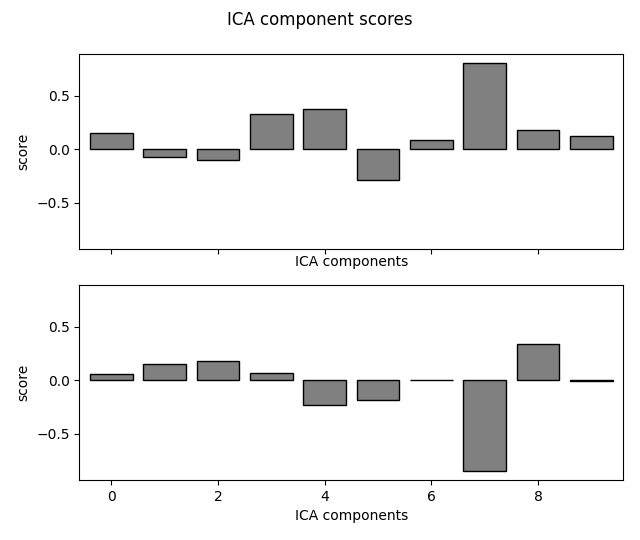
\includegraphics[height=0.6\textwidth]{images/obci_ica_scores.png}
    \caption{Scores of each ICA component for measurement from OpenBCI. The first row is in reference to the electrode \textit{Fp1} and the second row is in reference to the electrode \textit{Fp2}}
    \label{fig:obci_ica_scores}
\end{center}
\end{figure}

Generally a component with a score of more than 0.5 can be considered an artifact and hence can be removed from the measured signal. The two plots represent the scores with respect to the two reference electrode. Here component 7 is removed and the resulting EEG signal is given in the figure \ref{fig:obci_ica_overay}.

\begin{figure}[h] 
    \begin{center}
    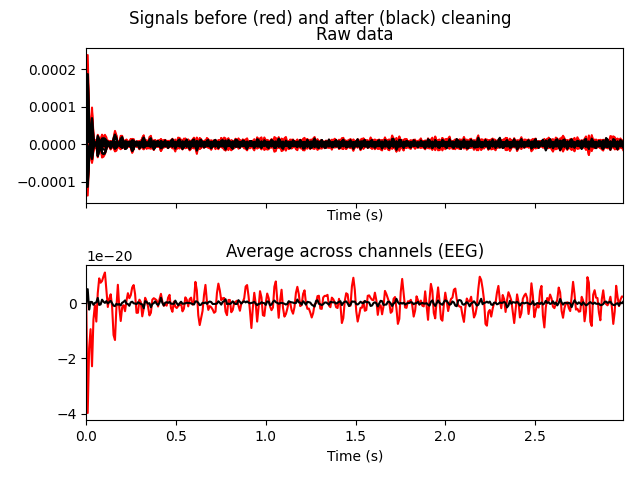
\includegraphics[height=0.6\textwidth]{images/obci_ica_overay.png}
    \caption{EEG signal before and after ICA component(artifact) removal}
    \label{fig:obci_ica_overay}
\end{center}
\end{figure}

 
\subsubsection{Signal Space Projection (SSP)}
SSP \nomenclature{SSP}{Signal Space Projection} helps in removing the artifacts in the signal by estimating a projection matrix based on measurements with and without signals of interest. The measurements are first taken without a subject to determine the directions of the noise vectors and the matrix formed by the noise vectors is used to project the measurement onto the hyperplane orthogonal to the noise vectors to remove the noise from the measurement data. Noise reduction leads to loss of dimensions however it is relatively less compared to the original signal space. The Raw data with SSP projections removed is shown in figure \ref{fig:obci_ssp}.

\begin{figure}[H] 
    \begin{center}
    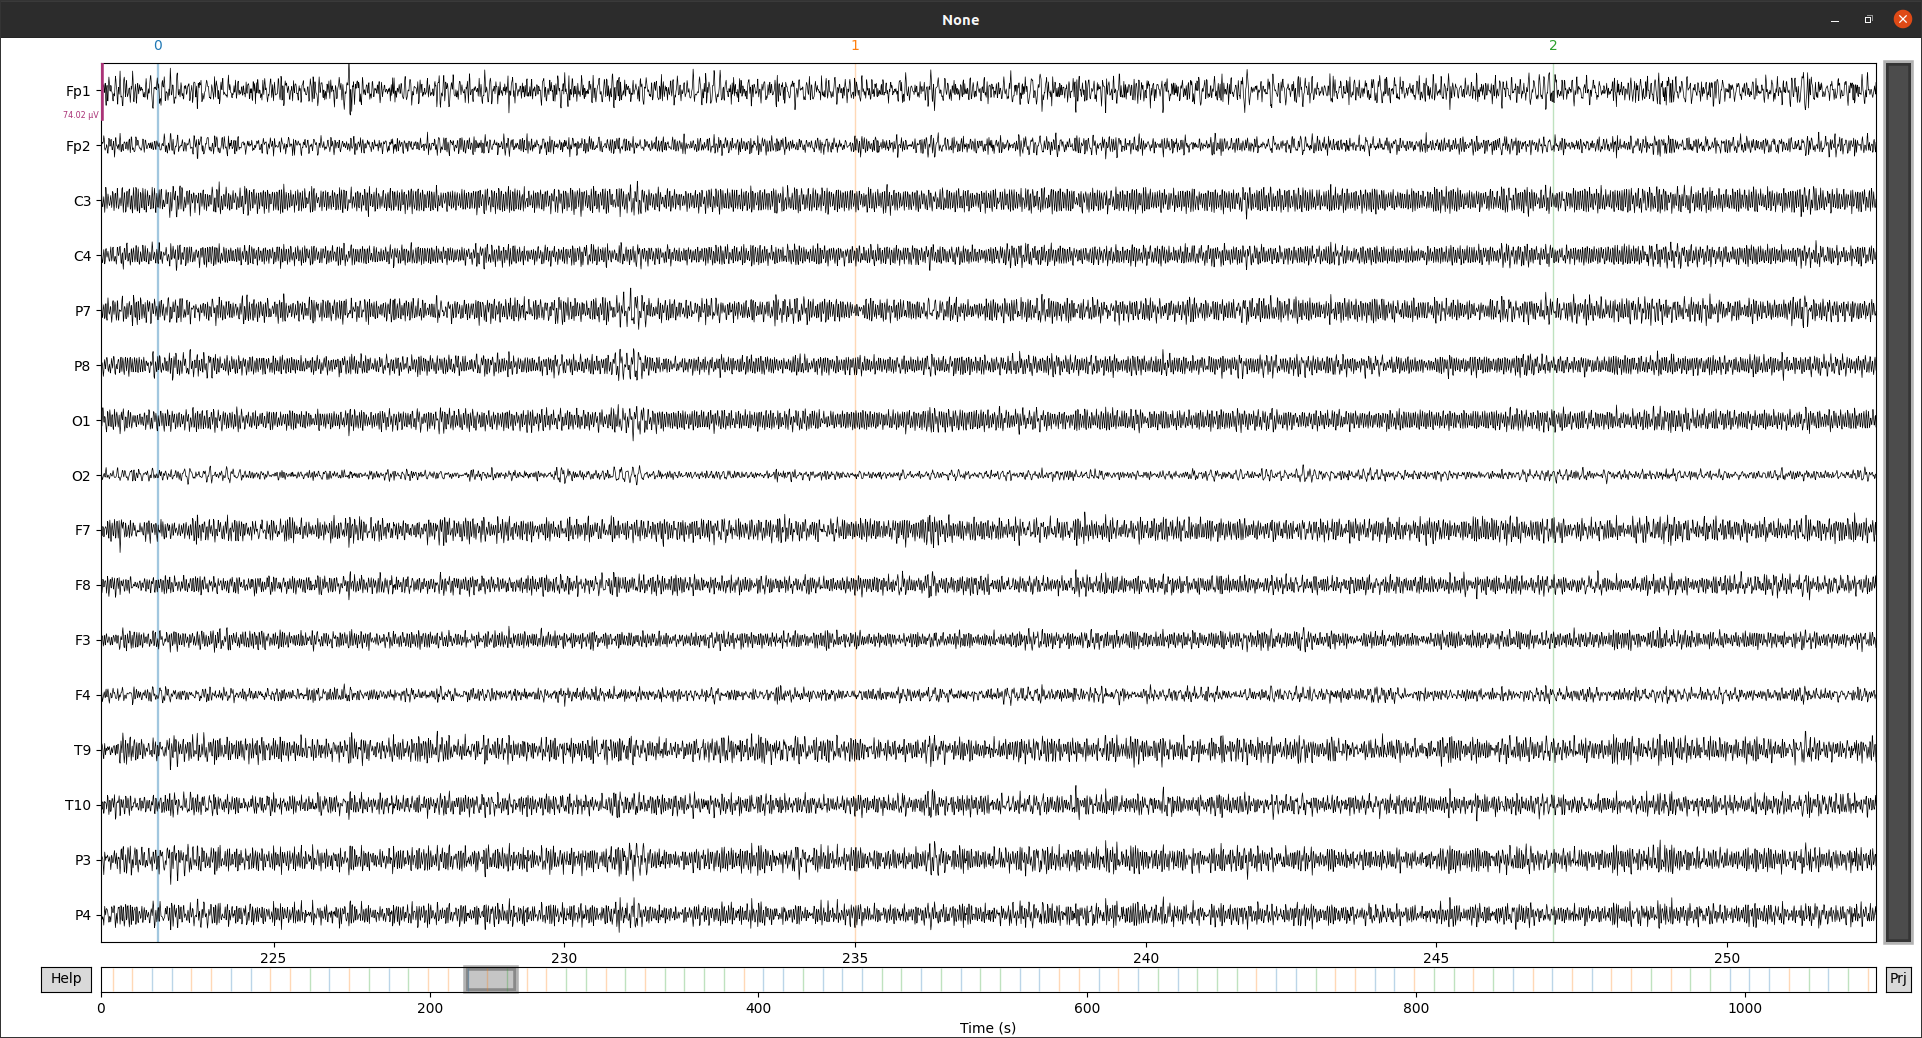
\includegraphics[height=0.6\textwidth]{images/obci_ssp.png}
    \caption{SSP projections applied on the EEG recording obtained from OpenBCI.The first image is before the application of the SSP projection and the second image is after application of SSP projection.}
    \label{fig:obci_ssp}
\end{center}
\end{figure}

\subsection{Epoch}
After preprocessing the measurement, the data that is stored in the RAW format cannot be used further for feature extraction or classification as it consists of information relating to all the classes, hence the data has to be broken down into segments with a specific time bound before and after the event, grouped together based on the class. This process is referred to as epoching. This enables extraction of distinctive features that are most prevalent in all the segments in a particular class. The data after epoching is of the shape $Ep \times N \times T$, where  $Ep$ is the number of epochs that is equal to the number of events, $N$ channels and $T$ epoched time points which is roughly between $-8$ and $4$ with the event trigger at the $0$ mark.

The frequency spectra of brain signals commonly have the $\frac{1}{f}$ structure, where the low frequency components dominate the results of the analysis. Power normalization resolves this by removing the $\frac{1}{f}$ and it is performed with the help of baselining the segments. Baseline is defined as a time interval usually before the occurrence of the event.

Power normalization is the ratio of activity (TF power) to baseline (TF power for a specific time window) \ref{eq:bell}.
\begin{equation} \label{eq:bell}
    10\log_{10}(\frac{activity}{baseline})
\end{equation}

Apart from power normalization, baselining helps in separating task from background activity, normally distributes the data and makes it easier to compare the values across individuals and frequencies. Epoch Image \ref{fig:obci_ep_image}visualizes the mean power across the channels for all the epochs.

\begin{figure}[H] 
    \begin{center}
    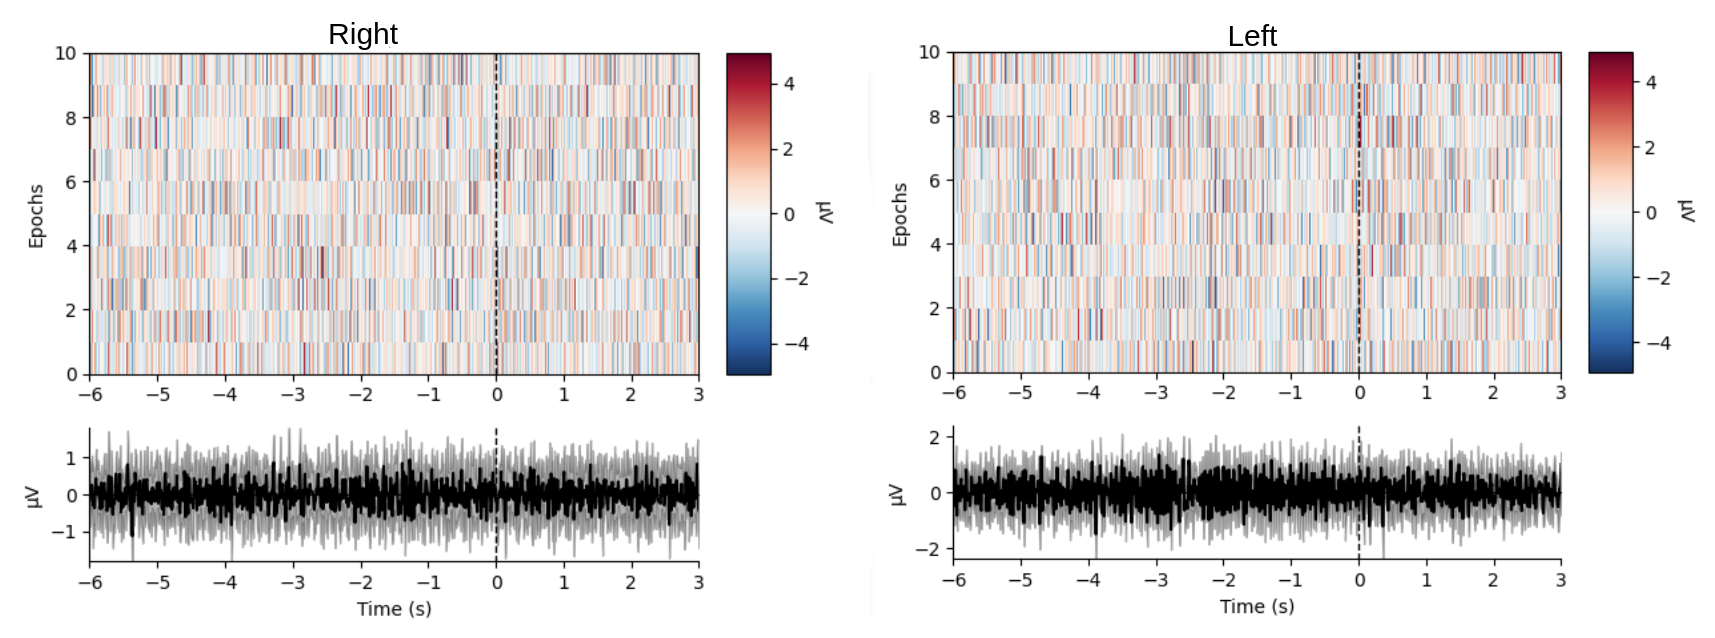
\includegraphics[width=1.0\textwidth]{images/Epoch_Image.png}
    \caption{Epoch image obtained from OpenBCI}
    \label{fig:obci_ep_image}
\end{center}
\end{figure}

The mean of epoch data for a particular event is called as Evoked data. It provides more insights such as event related topographical information (see figure \ref{fig:obci_evk_topo}).

\begin{figure}[H] 
    \begin{center}
    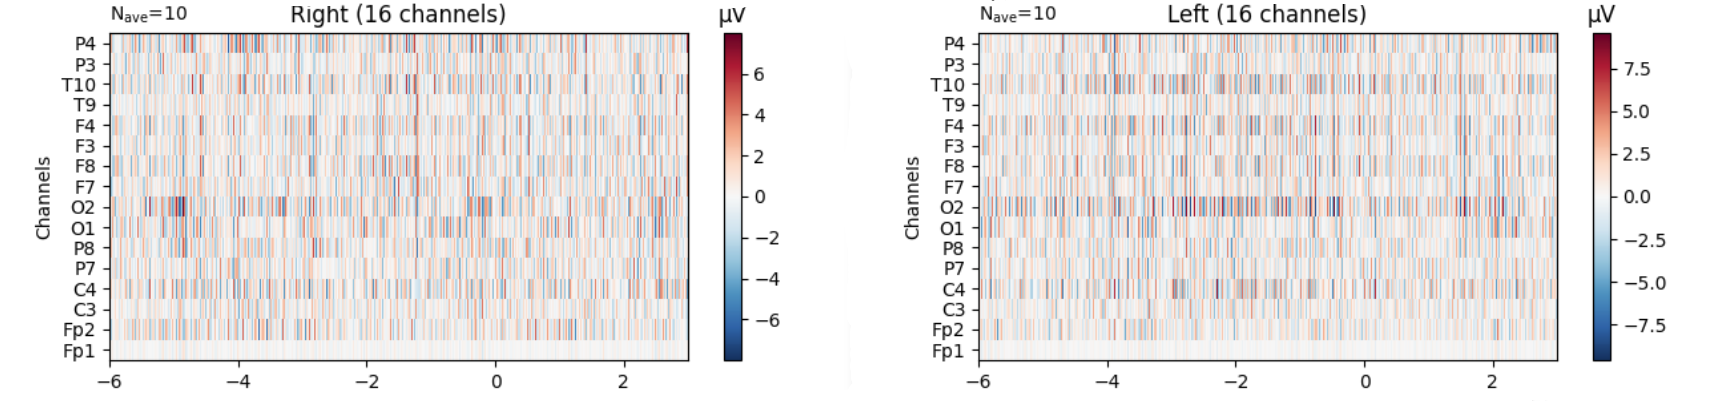
\includegraphics[width=1.0\textwidth]{images/evk_image.png}
    \caption{Evoked image obtained from OpenBCI}
    \label{fig:obci_evk_topo}
\end{center}
\end{figure}

\subsection{Feature Extraction}
Several features such as temporal, statistical and similar can be extracted from noise-free epoched data. Different methods of extraction and analysis are detailed in section \ref{feat_ext}.

\subsection{Feature Selection}
With increasing number of channels and extractions of various features, the feature space is increasingly rich and can provide accurate results. However this increases the dimensionality of the feature space making it computationally expensive leading to lagging responses and over-fitting. Feature selection techniques help in identifying the most discriminative features between the classes. \cite{2017_MI_ML_SP} discusses about the feature selection methods such as Minimum-redundancy and Maximum -relevance that selected features such as band power, wavelet energy, kurtosis and Lasso regularization that selects features such as band power, wavelet energy and auto-regressive coefficients.

As this work deals only with a 16-channel EEG system and less number of features, feature selection was not essential.

\subsection{Classification}
Machine Learning plays a predominant role in classification of the selected features. The models are trained on the selected features during the calibration and training phase. During online trials, the pre-trained classifiers are used in classification. Some of the commonly used classifiers are Support Vector Machines and Linear Discriminant Analysis, this is discussed further in section \ref{clasff}.

\section{Summary}
The clean data thus obtained are fed further down the pipeline where conventional approaches and deep learning approaches are used separately. The next chapter discusses conventional signal processing algorithms used in feature extraction. All the methods discussed are implemented and a comparative analysis and its results are discussed in the final chapter.